\section{Metodologi Eksperimen}

Setiap konfigurasi dijalankan 3 kali (\textit{seed} 1, 2, 3) pada ketiga instans.
Setiap pasangan (konfigurasi, \textit{seed}) mendapat \textit{seed} acak tersendiri yang
diturunkan dari nama konfigurasinya (\texttt{run\_seed}). Dengan demikian, misalnya,
GA 50 generasi bukan potongan awal dari GA 200 generasi, dan setiap \textit{run}
dapat direproduksi persis. Durasi diukur dengan \texttt{time.perf\_counter} untuk satu
\textit{run} dalam satu proses Python. Seluruh angka pada bab ini diambil dari
\texttt{output/*/*/summary.csv}. Folder setiap \textit{run} berisi \textit{state} awal
dan akhir (JSON dan gambar 3D) serta plot objektif terhadap iterasi.

Kolom \textbf{gap} adalah $1-f(s)/\text{batas atas}$ (Subbab~\ref{sec:bound}), yaitu
batas atas jarak hasil ke optimum global. Gap 0\% berarti hasilnya terbukti optimum global.

\section{Hasil Hill-Climbing}

Tabel~\ref{tab:hc-summary} merangkum keempat varian. Hasil setiap \textit{run}, termasuk
banyak iterasi, alasan berhenti, serta banyak \textit{restart} dan iterasi per
\textit{restart}, ada pada Tabel~\ref{tab:hc-runs}.

\begin{table}[H]\centering\small
\caption{Ringkasan Hill-Climbing (rata-rata 3 \textit{run})}\label{tab:hc-summary}
\begin{adjustbox}{max width=\textwidth}\begin{tabular}{l l r r r r r}
\toprule
\textbf{Instans} & \textbf{Varian} & \textbf{Akhir (mean $\pm$ std)} & \textbf{Min--maks} & \textbf{Gap (\%)} & \textbf{Durasi (s)} & \textbf{Iterasi} \\
\midrule
\multirow{4}{*}{\textit{small}} & Steepest & 680.7 $\pm$ 24.4 & 661--708 & 7.3 & 0.29 & 8.3 \\
 & Stochastic & 538.3 $\pm$ 115.0 & 406--614 & 26.7 & 0.03 & 7.0 \\
 & Sideways & 682.0 $\pm$ 45.0 & 630--708 & 7.1 & 1.18 & 28.7 \\
 & Random-restart & 712.7 $\pm$ 8.1 & 708--722 & 2.9 & 1.21 & 40.7 \\
\midrule
\multirow{4}{*}{\textit{medium}} & Steepest & 2213.7 $\pm$ 23.9 & 2197--2241 & 7.1 & 53.51 & 29.3 \\
 & Stochastic & 1469.7 $\pm$ 58.4 & 1404--1516 & 38.4 & 0.29 & 23.7 \\
 & Sideways & 2192.7 $\pm$ 12.7 & 2178--2201 & 8.0 & 50.77 & 47.7 \\
 & Random-restart & 2260.7 $\pm$ 7.2 & 2256--2269 & 5.2 & 120.72 & 167.7 \\
\midrule
\multirow{4}{*}{\textit{large}} & Steepest & 5205.7 $\pm$ 21.6 & 5181--5221 & 7.6 & 693.51 & 64.0 \\
 & Stochastic & 3061.0 $\pm$ 163.6 & 2912--3236 & 45.7 & 0.81 & 41.0 \\
 & Sideways & 5179.7 $\pm$ 91.9 & 5107--5283 & 8.0 & 922.48 & 82.3 \\
 & Random-restart & 5261.7 $\pm$ 46.1 & 5209--5295 & 6.6 & 1683.70 & 186.3 \\
\bottomrule
\end{tabular}\end{adjustbox}
\end{table}


\begin{figure}[H]
	\centering
	\begin{subfigure}{0.49\textwidth}
		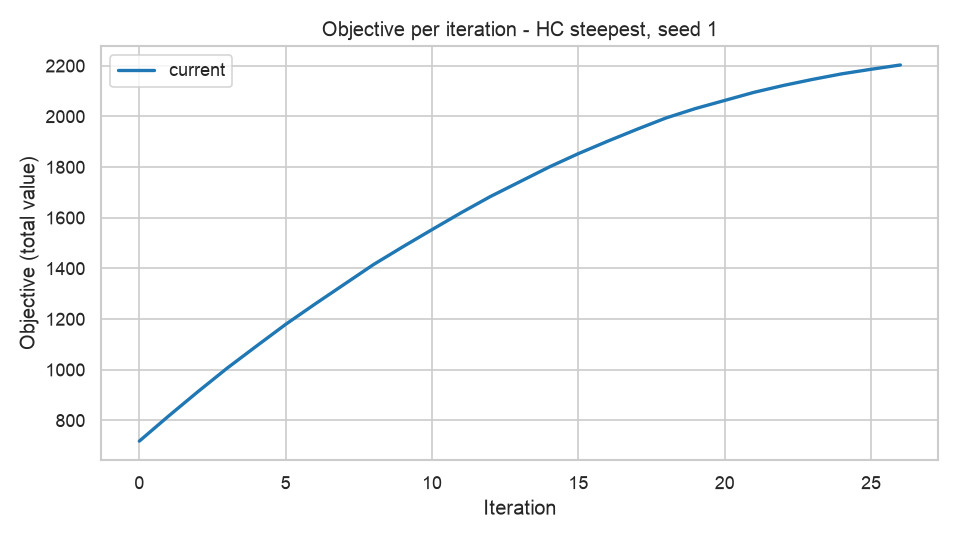
\includegraphics[width=\textwidth]{hc/medium/steepest/seed1/curve.png}
		\caption{\textit{Steepest-ascent}}
	\end{subfigure}
	\begin{subfigure}{0.49\textwidth}
		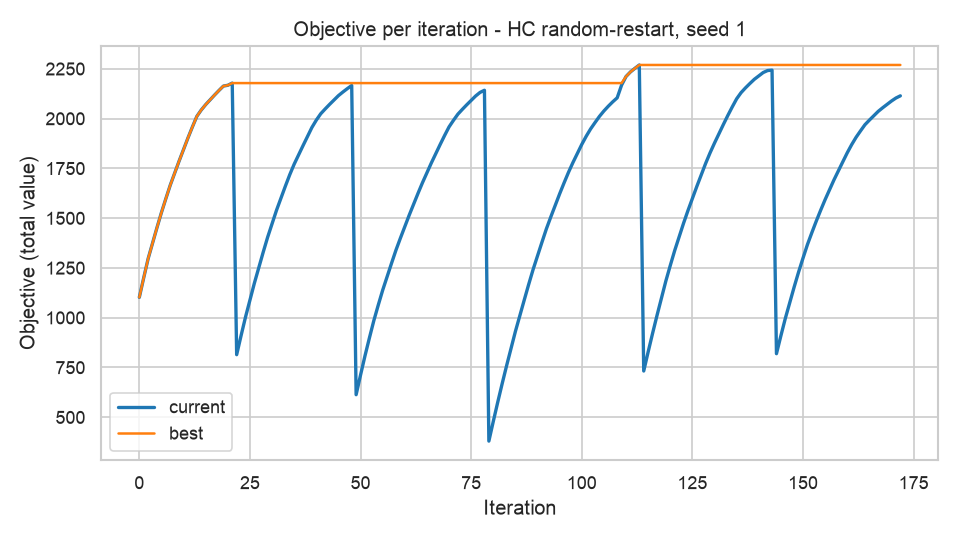
\includegraphics[width=\textwidth]{hc/medium/random-restart/seed1/curve.png}
		\caption{\textit{Random-restart}}
	\end{subfigure}
	\caption{Nilai objektif terhadap iterasi Hill-Climbing (instans \textit{medium}, \textit{seed} 1)}
	\label{fig:hc-curve}
\end{figure}

\begin{figure}[H]
	\centering
	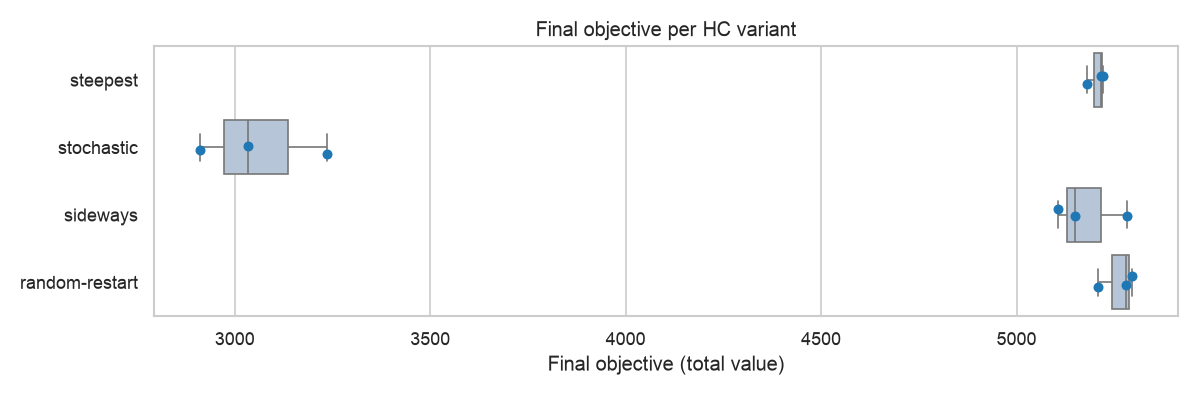
\includegraphics[width=0.75\textwidth]{hc/large/final_value_box.png}
	\caption{Sebaran nilai akhir varian Hill-Climbing (instans \textit{large})}
	\label{fig:hc-box}
\end{figure}

{\scriptsize\setlength{\tabcolsep}{4pt}
\begin{longtable}{l c r r r r r p{3.6cm}}
\caption{Hasil setiap \textit{run} Hill-Climbing}\label{tab:hc-runs}\\
\toprule
\textbf{Varian} & \textbf{Seed} & \textbf{Awal} & \textbf{Akhir} & \textbf{Gap (\%)} & \textbf{Durasi (s)} & \textbf{Iterasi} & \textbf{Berhenti karena} \\
\endfirsthead
\toprule
\textbf{Varian} & \textbf{Seed} & \textbf{Awal} & \textbf{Akhir} & \textbf{Gap (\%)} & \textbf{Durasi (s)} & \textbf{Iterasi} & \textbf{Berhenti karena} \\
\endhead
\midrule
\multicolumn{8}{l}{\textit{small} (batas atas 734)} \\
Steepest & 1 & 119 & 708 & 3.5 & 0.17 & 11 & local optimum \\
Steepest & 2 & 222 & 661 & 10.0 & 0.20 & 7 & local optimum \\
Steepest & 3 & 209 & 673 & 8.3 & 0.49 & 7 & local optimum \\
Stochastic & 1 & 270 & 615 & 16.2 & 0.10 & 10 & local optimum \\
Stochastic & 2 & 347 & 708 & 3.5 & 0.09 & 13 & local optimum \\
Stochastic & 3 & 317 & 708 & 3.5 & 0.10 & 10 & local optimum \\
Sideways & 1 & 235 & 630 & 14.2 & 1.27 & 27 & max sideways \\
Sideways & 2 & 189 & 708 & 3.5 & 1.20 & 29 & max sideways \\
Sideways & 3 & 279 & 708 & 3.5 & 1.07 & 30 & max sideways \\
Random-restart & 1 & 434 & 708 & 3.5 & 0.99 & 37 & max restart (5 restart: 4, 8, 7, 7, 5, 6) \\
Random-restart & 2 & 151 & 722 & 1.6 & 1.28 & 46 & max restart (5 restart: 8, 6, 9, 4, 10, 9) \\
Random-restart & 3 & 212 & 708 & 3.5 & 1.36 & 39 & max restart (5 restart: 8, 7, 6, 3, 7, 8) \\
\midrule
\multicolumn{8}{l}{\textit{medium} (batas atas 2384)} \\
Steepest & 1 & 718 & 2203 & 7.6 & 49.65 & 26 & local optimum \\
Steepest & 2 & 532 & 2197 & 7.8 & 86.02 & 31 & local optimum \\
Steepest & 3 & 602 & 2241 & 6.0 & 24.84 & 31 & local optimum \\
Stochastic & 1 & 944 & 2132 & 10.6 & 17.81 & 36 & local optimum \\
Stochastic & 2 & 361 & 2144 & 10.1 & 23.74 & 62 & local optimum \\
Stochastic & 3 & 674 & 2040 & 14.4 & 16.71 & 46 & local optimum \\
Sideways & 1 & 704 & 2199 & 7.8 & 49.59 & 47 & max sideways \\
Sideways & 2 & 732 & 2201 & 7.7 & 50.30 & 48 & max sideways \\
Sideways & 3 & 658 & 2178 & 8.6 & 52.40 & 48 & max sideways \\
Random-restart & 1 & 1102 & 2269 & 4.8 & 126.60 & 167 & max restart (5 restart: 21, 26, 29, 34, 29, 28) \\
Random-restart & 2 & 702 & 2256 & 5.4 & 117.72 & 163 & max restart (5 restart: 30, 29, 30, 23, 27, 24) \\
Random-restart & 3 & 794 & 2257 & 5.3 & 117.85 & 173 & max restart (5 restart: 28, 31, 27, 33, 28, 26) \\
\midrule
\multicolumn{8}{l}{\textit{large} (batas atas 5633)} \\
Steepest & 1 & 1485 & 5221 & 7.3 & 878.74 & 65 & local optimum \\
Steepest & 2 & 1379 & 5181 & 8.0 & 579.39 & 64 & local optimum \\
Steepest & 3 & 1506 & 5215 & 7.4 & 622.42 & 63 & local optimum \\
Stochastic & 1 & 1443 & 4585 & 18.6 & 441.50 & 100 & max iterasi \\
Stochastic & 2 & 1668 & 4792 & 14.9 & 800.63 & 96 & local optimum \\
Stochastic & 3 & 1475 & 4572 & 18.8 & 560.71 & 100 & max iterasi \\
Sideways & 1 & 1644 & 5107 & 9.3 & 934.22 & 82 & max sideways \\
Sideways & 2 & 1584 & 5283 & 6.2 & 838.40 & 81 & max sideways \\
Sideways & 3 & 1689 & 5149 & 8.6 & 994.83 & 84 & max sideways \\
Random-restart & 1 & 1989 & 5281 & 6.2 & 1654.99 & 185 & max restart (2 restart: 52, 67, 66) \\
Random-restart & 2 & 1329 & 5295 & 6.0 & 1698.62 & 189 & max restart (2 restart: 65, 59, 65) \\
Random-restart & 3 & 1586 & 5209 & 7.5 & 1697.51 & 185 & max restart (2 restart: 61, 61, 63) \\
\bottomrule
\end{longtable}
}


\section{Hasil Simulated Annealing}

Konfigurasi utama SA memakai jadwal geometrik, 20.000 iterasi, $p_0=0{,}01$, dan
$T_{\min}=0{,}05$ (Tabel~\ref{tab:sa-runs}). Gambar~\ref{fig:sa-curve} menunjukkan
plot objektif dan $e^{\Delta E/T}$ terhadap iterasi. Kolom \textbf{Stuck} adalah
frekuensi SA \textit{stuck} di \textit{local optimum}, yaitu banyaknya \textit{plateau}
dengan nilai objektif tidak berubah selama minimal 500 iterasi.

\begin{table}[H]\centering\small
\caption{Hasil setiap \textit{run} Simulated Annealing (geometrik, 20.000 iterasi, $p_0=0{,}01$, $T_{\min}=0{,}05$)}\label{tab:sa-runs}
\begin{adjustbox}{max width=\textwidth}\begin{tabular}{c r r r r r r r}
\toprule
\textbf{Seed} & \textbf{Awal} & \textbf{Akhir} & \textbf{Gap (\%)} & \textbf{Durasi (s)} & \textbf{$T_0$} & \textbf{Stuck} & \textbf{Iterasi terbaik} \\
\midrule
\multicolumn{8}{l}{\textit{small} (batas atas 734)} \\
1 & 244 & 734 & 0.0 & 4.62 & 9.28 & 4 & 11860 \\
2 & 94 & 734 & 0.0 & 4.75 & 9.19 & 1 & 776 \\
3 & 289 & 734 & 0.0 & 4.53 & 15.12 & 3 & 8718 \\
\midrule
\multicolumn{8}{l}{\textit{medium} (batas atas 2384)} \\
1 & 899 & 2248 & 5.7 & 23.12 & 12.47 & 4 & 12907 \\
2 & 710 & 2209 & 7.3 & 23.24 & 12.08 & 7 & 19857 \\
3 & 639 & 2243 & 5.9 & 22.75 & 9.83 & 8 & 15616 \\
\midrule
\multicolumn{8}{l}{\textit{large} (batas atas 5633)} \\
1 & 1669 & 4932 & 12.4 & 21.09 & 11.17 & 7 & 18777 \\
2 & 1505 & 4943 & 12.2 & 21.87 & 8.11 & 11 & 18974 \\
3 & 1433 & 5053 & 10.3 & 21.56 & 9.66 & 7 & 16325 \\
\bottomrule
\end{tabular}\end{adjustbox}
\end{table}


\begin{figure}[H]
	\centering
	\begin{subfigure}{0.49\textwidth}
		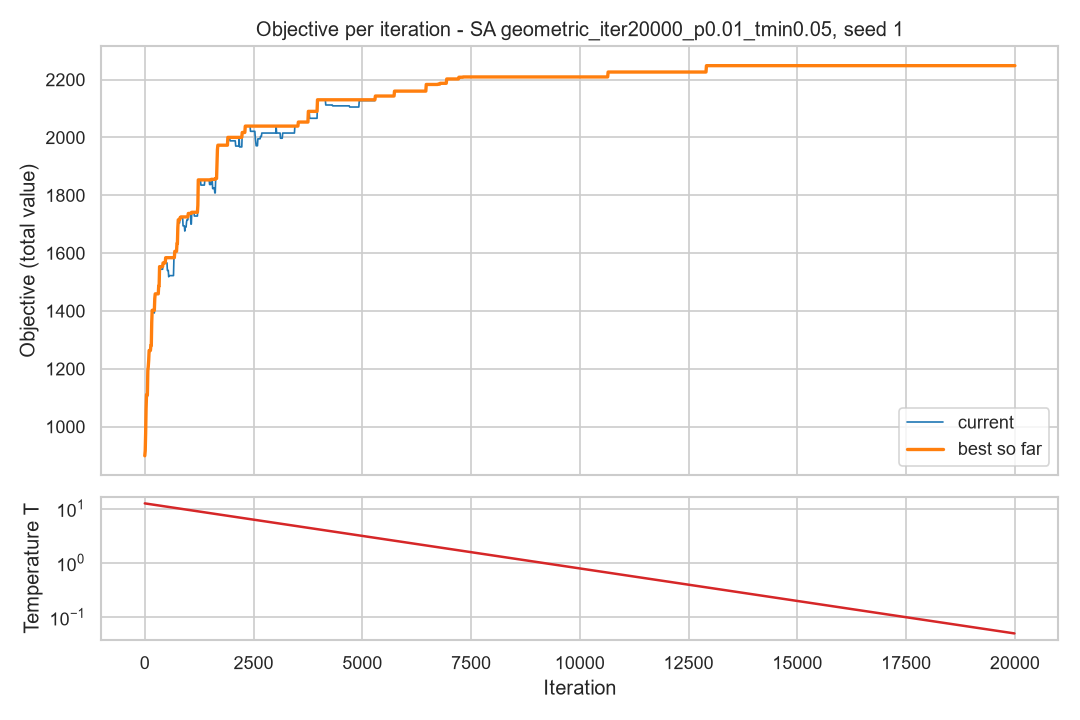
\includegraphics[width=\textwidth]{sa/medium/geometric_iter20000_p0.01_tmin0.05/seed1/curve.png}
		\caption{Nilai objektif dan suhu}
	\end{subfigure}
	\begin{subfigure}{0.49\textwidth}
		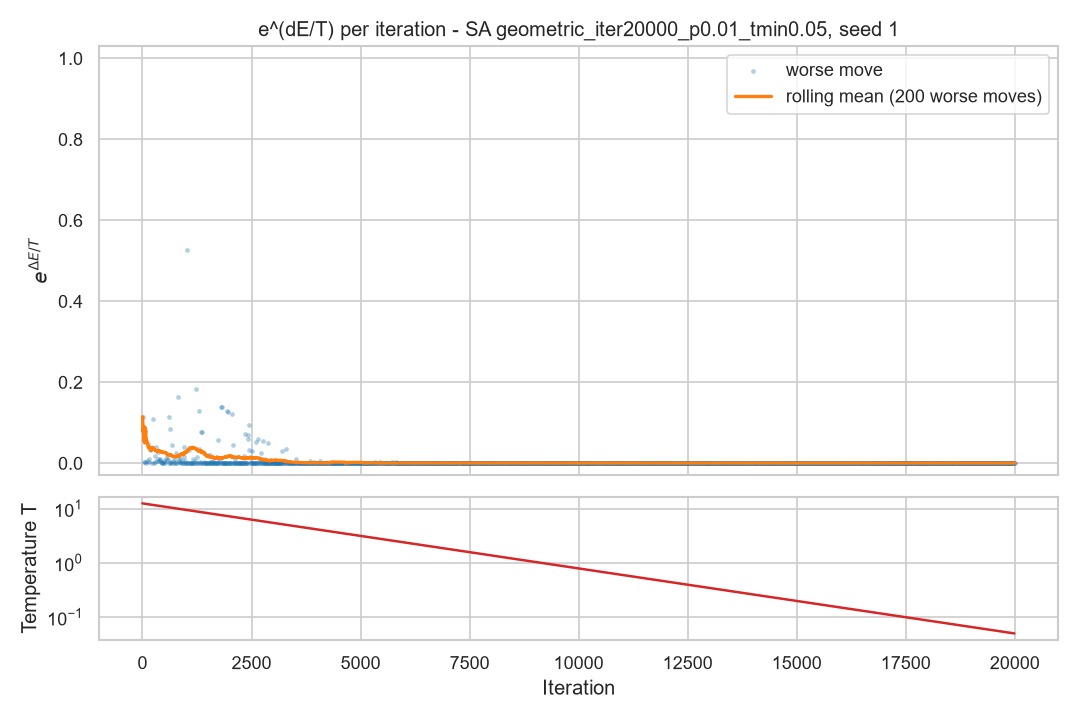
\includegraphics[width=\textwidth]{sa/medium/geometric_iter20000_p0.01_tmin0.05/seed1/eet.png}
		\caption{$e^{\Delta E/T}$}
	\end{subfigure}
	\caption{Simulated Annealing pada instans \textit{medium} (\textit{seed} 1)}
	\label{fig:sa-curve}
\end{figure}

Parameter SA juga diuji pada instans \textit{medium}, satu parameter divariasikan
setiap kali (Tabel~\ref{tab:sa-params}, Gambar~\ref{fig:sa-compare}).

\begin{table}[H]\centering\scriptsize
\caption{Pengaruh parameter Simulated Annealing pada instans \textit{medium} (rata-rata 3 \textit{run})}\label{tab:sa-params}
\begin{adjustbox}{max width=\textwidth}\begin{tabular}{l l r r r r r r r r}
\toprule
\textbf{Variasi} & \textbf{Jadwal} & \textbf{Iterasi} & \textbf{$p_0$} & \textbf{$T_{\min}$} & \textbf{Bias} & \textbf{Akhir} & \textbf{Gap (\%)} & \textbf{Durasi (s)} & \textbf{Stuck} \\
\midrule
\multirow{5}{*}{Iterasi} & geometric & 2500 & 0.8 & 0.05 & 0 & 1985.7 $\pm$ 41.5 & 16.7 & 1.7 & 0.0 \\
 & geometric & 5000 & 0.8 & 0.05 & 0 & 2075.7 $\pm$ 14.7 & 12.9 & 3.8 & 1.3 \\
 & geometric & 10000 & 0.8 & 0.05 & 0 & 2187.7 $\pm$ 49.0 & 8.2 & 8.4 & 2.7 \\
 & geometric & 20000 & 0.8 & 0.05 & 0 & 2226.0 $\pm$ 30.0 & 6.6 & 16.8 & 5.7 \\
 & geometric & 40000 & 0.8 & 0.05 & 0 & 2262.3 $\pm$ 13.2 & 5.1 & 37.3 & 10.0 \\
\midrule
\multirow{5}{*}{$p_0$} & geometric & 10000 & 0.01 & 0.05 & 0 & 2232.3 $\pm$ 18.6 & 6.4 & 10.7 & 5.0 \\
 & geometric & 10000 & 0.2 & 0.05 & 0 & 2163.3 $\pm$ 37.3 & 9.3 & 10.1 & 3.3 \\
 & geometric & 10000 & 0.5 & 0.05 & 0 & 2169.3 $\pm$ 39.1 & 9.0 & 8.9 & 3.3 \\
 & geometric & 10000 & 0.8 & 0.05 & 0 & 2187.7 $\pm$ 49.0 & 8.2 & 8.4 & 2.7 \\
 & geometric & 10000 & 0.95 & 0.05 & 0 & 2147.0 $\pm$ 13.5 & 9.9 & 7.6 & 2.3 \\
\midrule
\multirow{2}{*}{Jadwal} & geometric & 10000 & 0.8 & 0.05 & 0 & 2187.7 $\pm$ 49.0 & 8.2 & 8.4 & 2.7 \\
 & linear & 10000 & 0.8 & 0.05 & 0 & 1755.7 $\pm$ 69.0 & 26.4 & 3.3 & 0.0 \\
\midrule
\multirow{4}{*}{$T_{\min}$} & geometric & 10000 & 0.8 & 0.05 & 0 & 2187.7 $\pm$ 49.0 & 8.2 & 8.4 & 2.7 \\
 & geometric & 10000 & 0.8 & 0.5 & 0 & 2149.0 $\pm$ 79.1 & 9.9 & 8.0 & 2.7 \\
 & geometric & 10000 & 0.8 & 2 & 0 & 2132.3 $\pm$ 64.6 & 10.6 & 6.9 & 0.3 \\
 & geometric & 10000 & 0.8 & 5 & 0 & 1994.3 $\pm$ 17.2 & 16.3 & 5.6 & 0.3 \\
\midrule
\multirow{3}{*}{Ratio bias} & geometric & 20000 & 0.01 & 0.05 & 0 & 2233.3 $\pm$ 21.2 & 6.3 & 23.0 & 6.3 \\
 & geometric & 20000 & 0.01 & 0.05 & 0.2 & 2247.3 $\pm$ 35.0 & 5.7 & 22.4 & 5.7 \\
 & geometric & 20000 & 0.01 & 0.05 & 0.5 & 2251.7 $\pm$ 40.4 & 5.5 & 241.7 & 5.3 \\
\bottomrule
\end{tabular}\end{adjustbox}
\end{table}


Rata-rata durasi \textit{ratio bias} 0,5 pada Tabel~\ref{tab:sa-params} dipengaruhi satu
\textit{run} (\textit{seed} 1) yang tercatat 683 detik, padahal dua \textit{run} lainnya
sekitar 21 detik. Nilai objektifnya tidak terpengaruh.

\begin{figure}[H]
	\centering
	\begin{subfigure}{0.49\textwidth}
		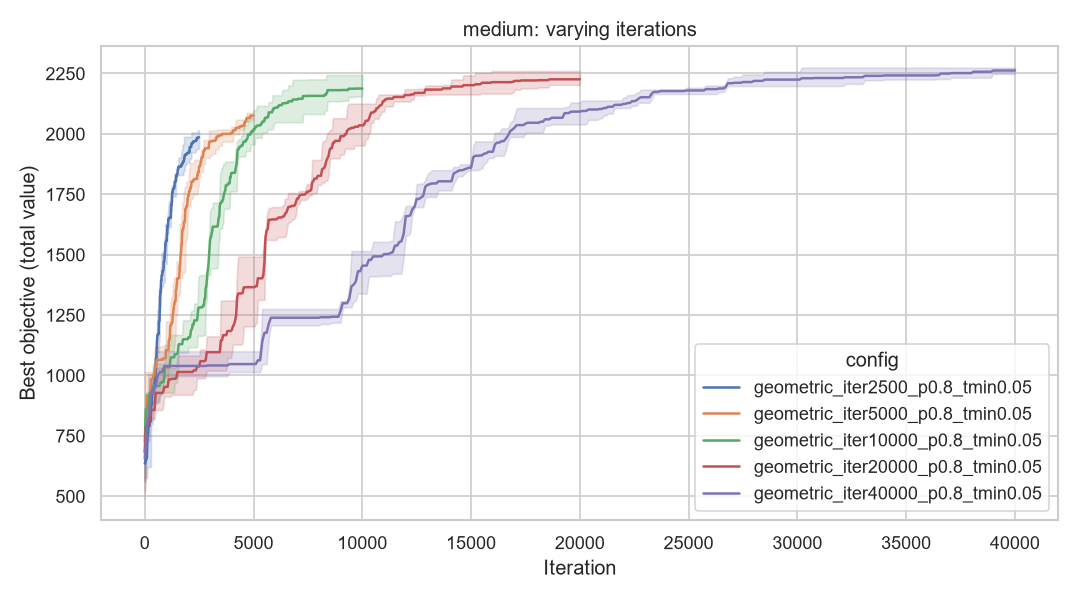
\includegraphics[width=\textwidth]{sa/medium/compare_iterations.png}
		\caption{Banyak iterasi}
	\end{subfigure}
	\begin{subfigure}{0.49\textwidth}
		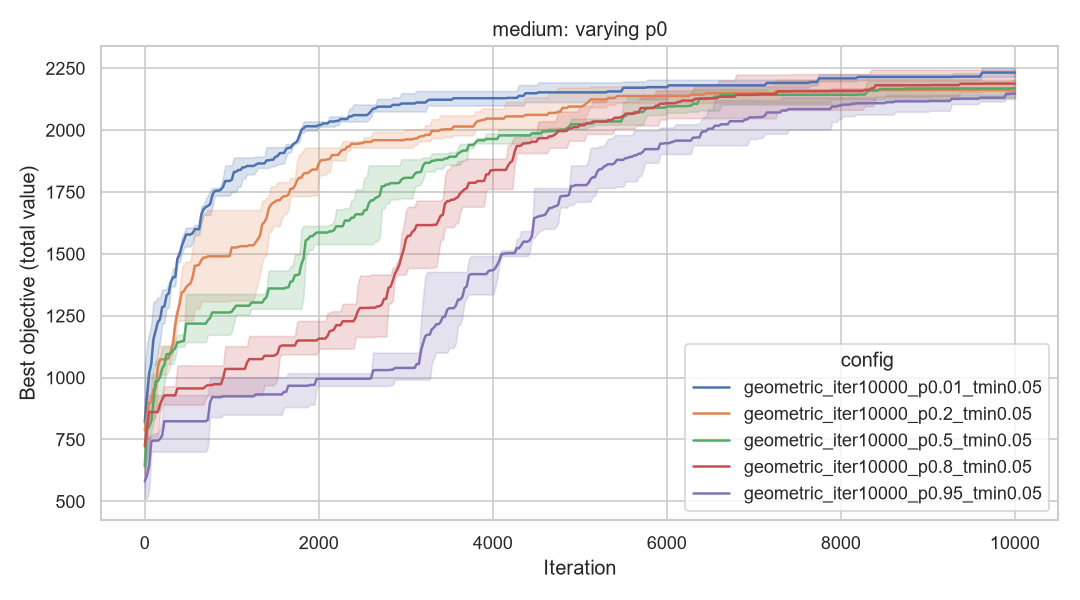
\includegraphics[width=\textwidth]{sa/medium/compare_p0.png}
		\caption{$p_0$}
	\end{subfigure}
	\begin{subfigure}{0.49\textwidth}
		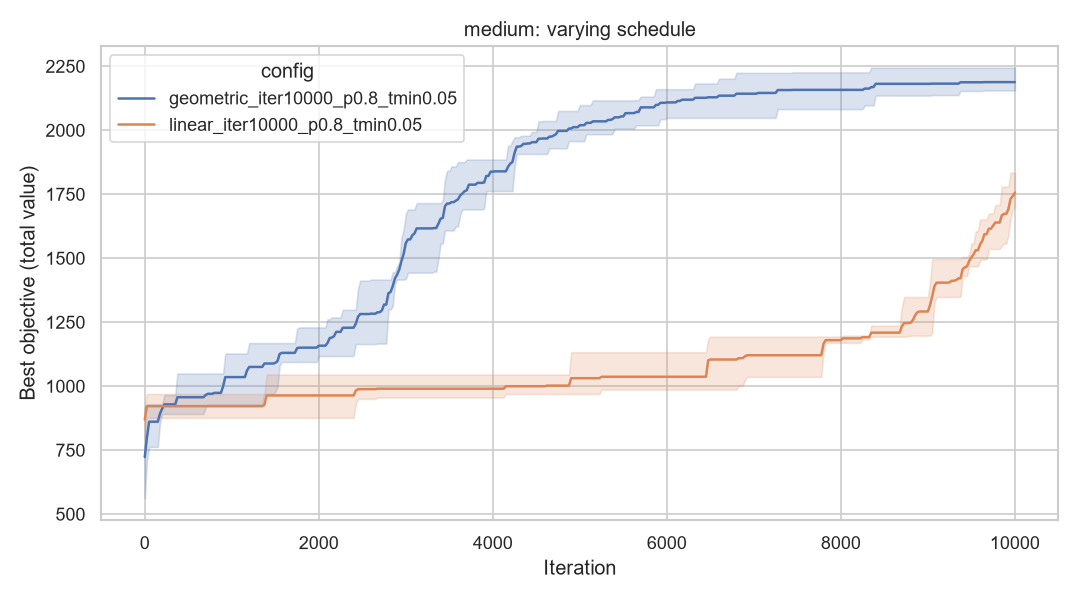
\includegraphics[width=\textwidth]{sa/medium/compare_schedule.png}
		\caption{Jadwal suhu}
	\end{subfigure}
	\begin{subfigure}{0.49\textwidth}
		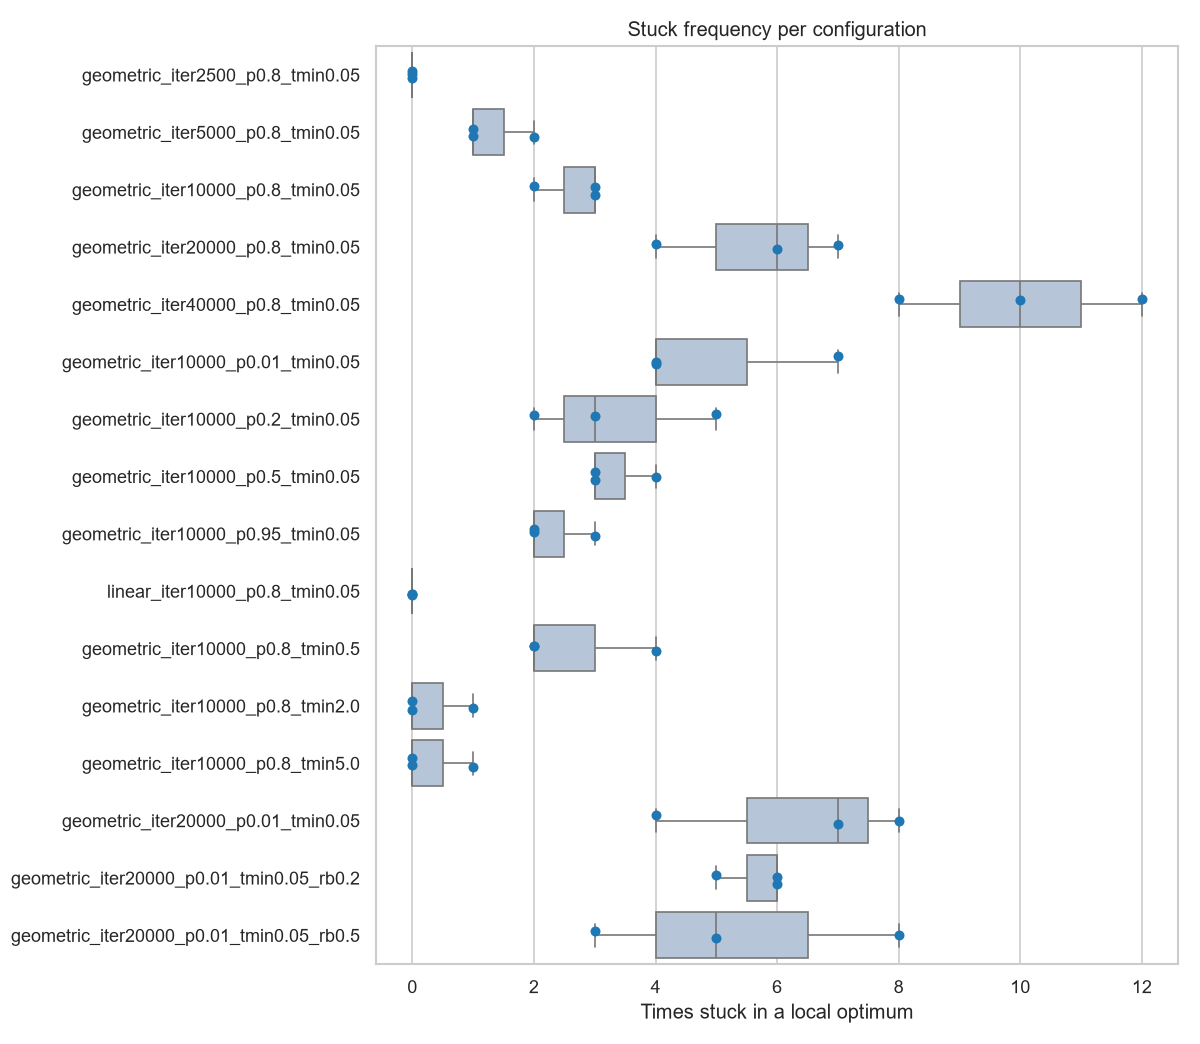
\includegraphics[width=\textwidth]{sa/medium/stuck_count_box.png}
		\caption{Frekuensi \textit{stuck}}
	\end{subfigure}
	\caption{Perbandingan konfigurasi Simulated Annealing (instans \textit{medium})}
	\label{fig:sa-compare}
\end{figure}

\begin{table}[H]\centering\small
\caption{Pengaruh \textit{ratio bias} pada instans \textit{large} (rata-rata 3 \textit{run})}\label{tab:sa-large-bias}
\begin{tabular}{r r r r r}
\toprule
\textbf{Ratio bias} & \textbf{Akhir} & \textbf{Gap (\%)} & \textbf{Durasi (s)} & \textbf{Stuck} \\
\midrule
0 & 4976.0 $\pm$ 66.9 & 11.7 & 21.5 & 8.3 \\
0.2 & 5076.3 $\pm$ 42.3 & 9.9 & 21.3 & 9.0 \\
0.5 & 5058.0 $\pm$ 74.8 & 10.2 & 19.7 & 8.0 \\
\bottomrule
\end{tabular}
\end{table}


\section{Hasil Genetic Algorithm}

Sesuai spesifikasi, dilakukan dua eksperimen: (1) populasi tetap 50 dengan
generasi 50, 100, dan 200; (2) generasi tetap 100 dengan populasi 20, 50, dan 100.
Laju mutasi 0,2 dan \textit{elitism} 1. Konfigurasi (50, 100) termasuk dalam kedua
eksperimen. Ringkasannya ada pada Tabel~\ref{tab:ga-summary}, sedangkan hasil setiap
\textit{run} (populasi, iterasi, nilai awal dan akhir, durasi) ada pada
Tabel~\ref{tab:ga-runs} di Lampiran. Kolom ``Awal'' adalah nilai individu terbaik
generasi ke-0.

\begin{table}[H]\centering\small
\caption{Ringkasan Genetic Algorithm (rata-rata 3 \textit{run})}\label{tab:ga-summary}
\begin{adjustbox}{max width=\textwidth}\begin{tabular}{l r r r r r r r r}
\toprule
\textbf{Instans} & \textbf{Pop.} & \textbf{Gen.} & \textbf{Awal} & \textbf{Akhir (mean $\pm$ std)} & \textbf{Min--maks} & \textbf{Gap (\%)} & \textbf{Durasi (s)} & \textbf{Gen. terbaik} \\
\midrule
\multirow{5}{*}{\textit{small}} & 50.0 & 50.0 & 488.3 & 608.0 $\pm$ 41.2 & 563--644 & 17.2 & 0.21 & 29.0 \\
 & 50.0 & 100.0 & 486.0 & 640.7 $\pm$ 12.0 & 629--653 & 12.7 & 0.38 & 61.0 \\
 & 50.0 & 200.0 & 380.7 & 698.3 $\pm$ 16.7 & 679--708 & 4.9 & 1.03 & 110.0 \\
 & 20.0 & 100.0 & 389.0 & 569.3 $\pm$ 26.5 & 548--599 & 22.4 & 0.20 & 64.0 \\
 & 100.0 & 100.0 & 437.0 & 655.3 $\pm$ 11.5 & 644--667 & 10.7 & 1.18 & 54.7 \\
\midrule
\multirow{5}{*}{\textit{medium}} & 50.0 & 50.0 & 1082.3 & 1221.7 $\pm$ 58.3 & 1186--1289 & 48.8 & 0.15 & 24.3 \\
 & 50.0 & 100.0 & 992.0 & 1319.3 $\pm$ 211.7 & 1154--1558 & 44.7 & 0.34 & 90.3 \\
 & 50.0 & 200.0 & 1034.7 & 1477.7 $\pm$ 105.2 & 1369--1579 & 38.0 & 0.67 & 185.3 \\
 & 20.0 & 100.0 & 975.0 & 1220.0 $\pm$ 98.1 & 1120--1316 & 48.8 & 0.13 & 89.7 \\
 & 100.0 & 100.0 & 993.3 & 1422.7 $\pm$ 78.7 & 1353--1508 & 40.3 & 0.63 & 91.3 \\
\midrule
\multirow{5}{*}{\textit{large}} & 50.0 & 50.0 & 2030.0 & 2080.0 $\pm$ 17.7 & 2064--2099 & 63.1 & 0.98 & 27.3 \\
 & 50.0 & 100.0 & 2074.7 & 2115.0 $\pm$ 245.5 & 1932--2394 & 62.5 & 2.42 & 14.0 \\
 & 50.0 & 200.0 & 1983.7 & 2096.3 $\pm$ 220.9 & 1923--2345 & 62.8 & 6.37 & 187.0 \\
 & 20.0 & 100.0 & 2070.0 & 2211.0 $\pm$ 112.9 & 2130--2340 & 60.7 & 1.29 & 91.3 \\
 & 100.0 & 100.0 & 2181.0 & 2265.7 $\pm$ 193.5 & 2071--2458 & 59.8 & 10.69 & 57.0 \\
\bottomrule
\end{tabular}\end{adjustbox}
\end{table}


\begin{figure}[H]
	\centering
	\begin{subfigure}{0.49\textwidth}
		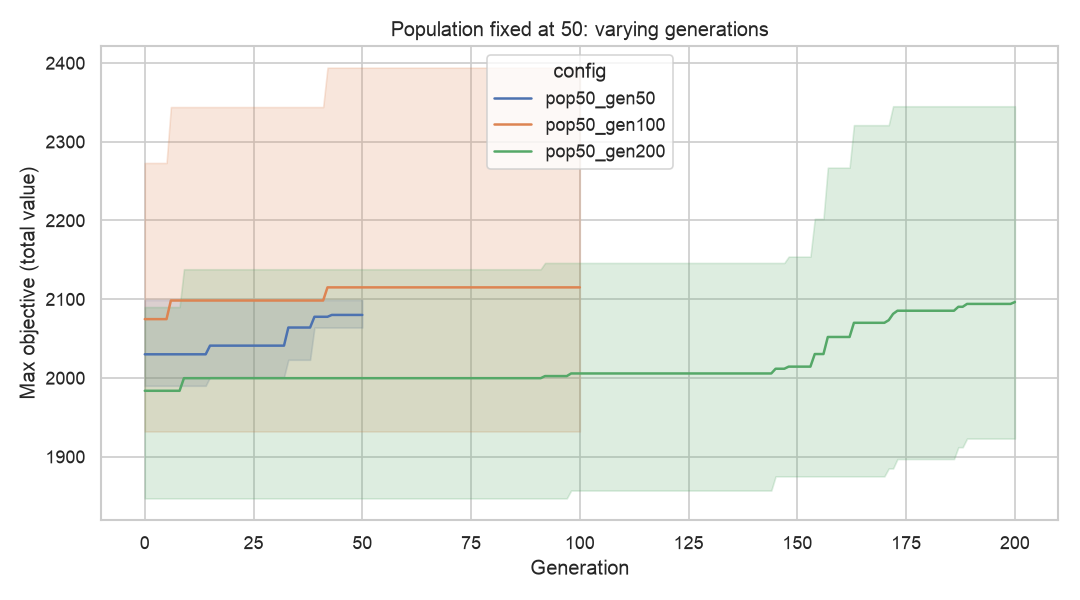
\includegraphics[width=\textwidth]{ga/large/compare_generations.png}
		\caption{Populasi 50, generasi bervariasi}
	\end{subfigure}
	\begin{subfigure}{0.49\textwidth}
		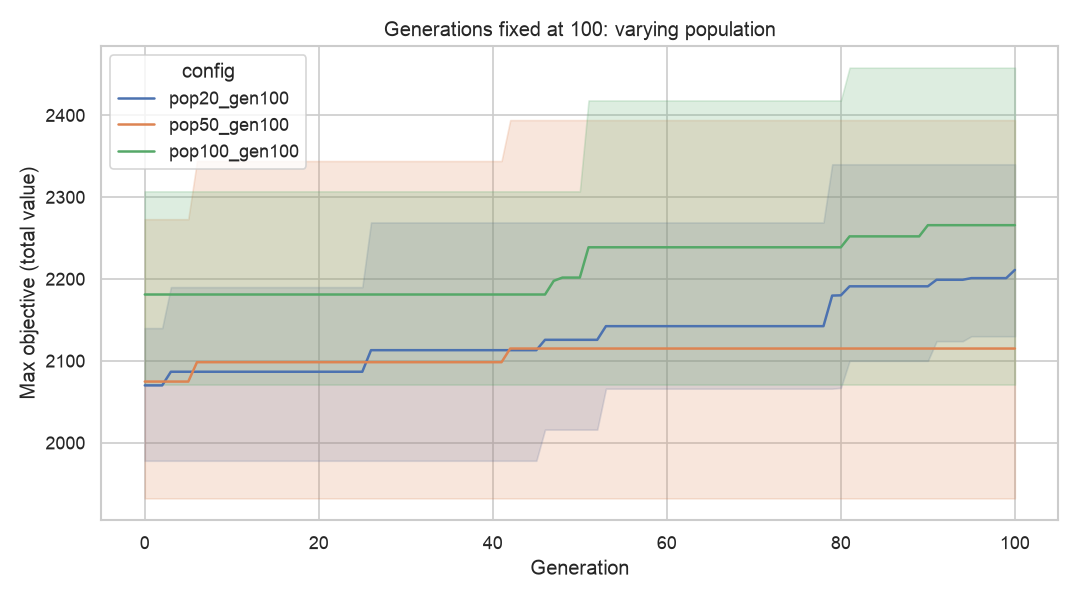
\includegraphics[width=\textwidth]{ga/large/compare_population.png}
		\caption{Generasi 100, populasi bervariasi}
	\end{subfigure}
	\caption{Nilai objektif maksimum GA terhadap generasi (instans \textit{large}; garis = rata-rata 3 \textit{run}, area = rentang)}
	\label{fig:ga-compare}
\end{figure}

\begin{figure}[H]
	\centering
	\begin{subfigure}{0.49\textwidth}
		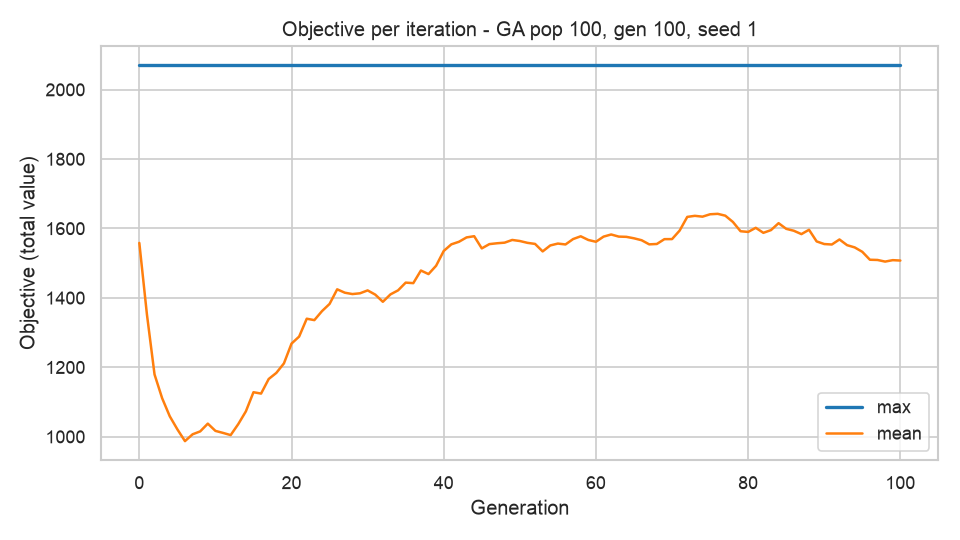
\includegraphics[width=\textwidth]{ga/large/pop100_gen100/seed1/curve.png}
		\caption{Nilai maksimum dan rata-rata populasi}
	\end{subfigure}
	\begin{subfigure}{0.49\textwidth}
		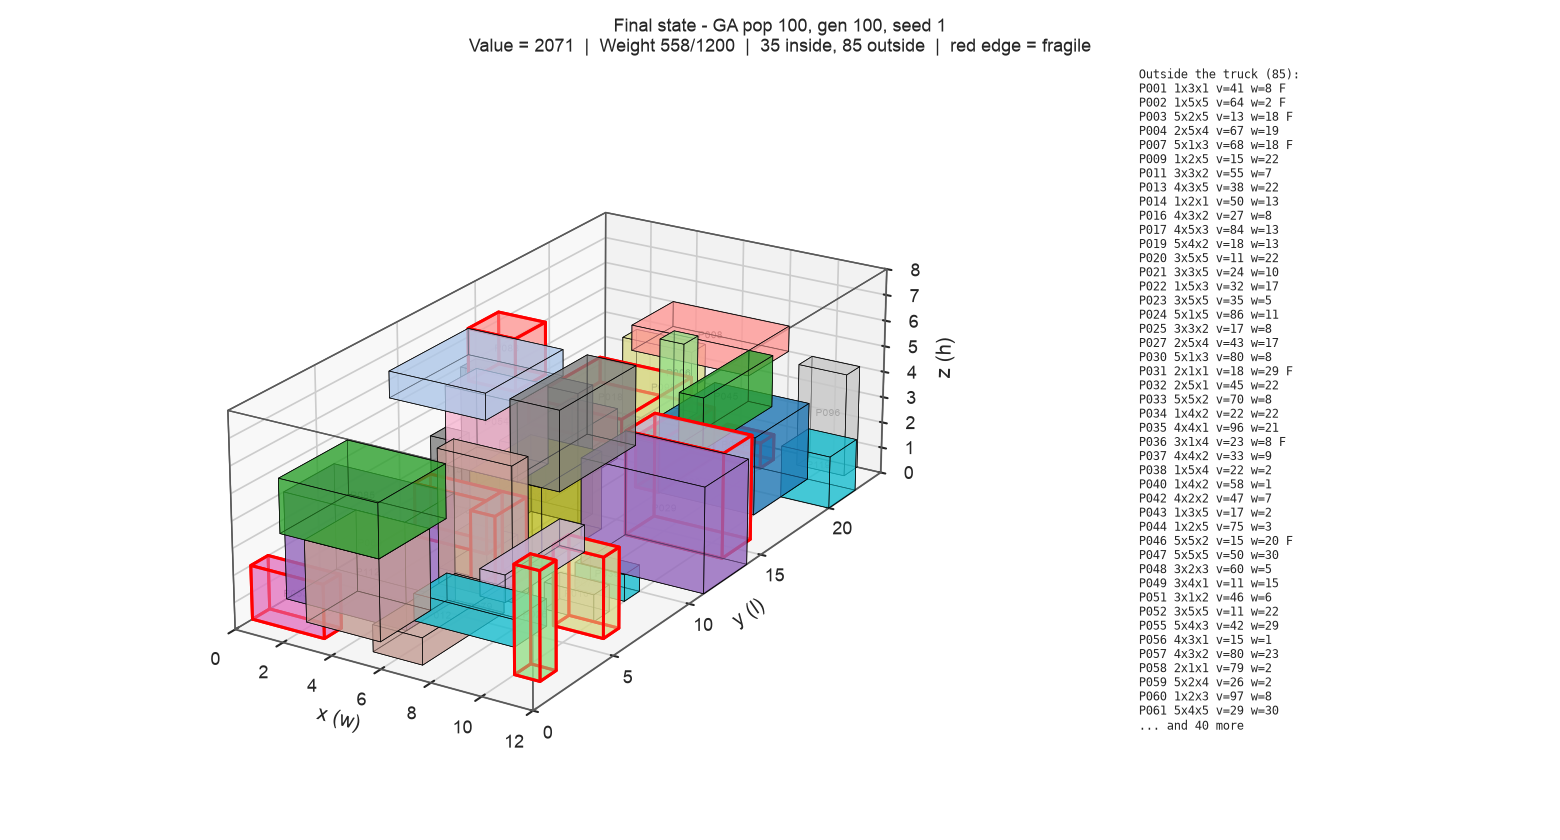
\includegraphics[width=\textwidth]{ga/large/pop100_gen100/seed1/final.png}
		\caption{\textit{State} akhir}
	\end{subfigure}
	\caption{GA populasi 100, generasi 100 (instans \textit{large}, \textit{seed} 1)}
	\label{fig:ga-run}
\end{figure}

\section{Hasil Bonus: Objektif ETA}

SA (jadwal geometrik, 20.000 iterasi, $p_0=0{,}01$, \textit{seed} 1) dijalankan pada
instans \textit{medium} dengan objektif ETA dan objektif \textit{value} biasa
(\texttt{output/sa/medium/eta/}).

\begin{table}[H]
	\centering
	\caption{Perbandingan objektif \textit{value} dan ETA (SA, instans \textit{medium}, \textit{seed} 1)}
	\label{tab:eta}
	\begin{tabular}{l r r r r}
		\toprule
		\textbf{Objektif} & \textbf{Total value} & $\sum$ \textbf{value/ETA} & \textbf{Paket dimuat} & \textbf{Rata-rata ETA} \\
		\midrule
		\textit{value} & 2266 & 933,4 & 40 & 3,95 \\
		ETA & 2180 & 966,0 & 40 & 3,70 \\
		\bottomrule
	\end{tabular}
\end{table}

Objektif ETA mengorbankan 3,8\% total \textit{value} untuk memuat paket dengan rata-rata
ETA lebih kecil (3,70 dibanding 3,95 hari; rata-rata ETA semua paket 4,11). Artinya,
paket yang lebih mendesak lebih diprioritaskan, sesuai tujuan objektif ini.

\section{Hasil Bonus: Multi-Truk}
\label{sec:multitruck-hasil}

Armada dua truk identik diuji pada instans \textit{medium} dan \textit{large} dengan
parameter yang sama seperti eksperimen satu truk (3 \textit{run} per konfigurasi;
hasilnya ada di \texttt{output/*/medium\_trucks2/} dan \texttt{output/*/large\_trucks2/}).
HC hanya dijalankan untuk \textit{steepest} dan \textit{stochastic} di \textit{medium}
karena waktu eksekusinya. Untuk kedua instans, total berat dan volume seluruh paket
muat di dua truk, sehingga batas atasnya sama dengan total \textit{value} semua paket
(2608 dan 6194). Seluruh 42 \textit{state} akhir diperiksa ulang dengan pemeriksa
independen berbasis sel, dan semuanya valid.

\begin{table}[H]
	\centering
	\caption{Hasil multi-truk dibanding satu truk (rata-rata 3 \textit{run})}
	\label{tab:multitruck}
	\begin{adjustbox}{max width=\textwidth}
	\begin{tabular}{l l r r r r}
		\toprule
		\textbf{Instans} & \textbf{Algoritma} & \textbf{1 truk} & \textbf{2 truk (mean $\pm$ std)} & \textbf{Gap 2 truk (\%)} & \textbf{Durasi 2 truk (s)} \\
		\midrule
		\multirow{5}{*}{\textit{medium}} & HC \textit{steepest} & 2213,7 & 2544,3 $\pm$ 6,5 & 2,4 & 48,1 \\
		& HC \textit{stochastic} & 2105,3 & 2426,0 $\pm$ 51,6 & 7,0 & 23,7 \\
		& SA (20.000 iterasi, $p_0=0{,}01$) & 2233,3 & 2543,0 $\pm$ 28,0 & 2,5 & 4,6 \\
		& GA (pop. 50, gen. 100) & 1319,3 & 1608,7 $\pm$ 66,3 & 38,3 & 0,7 \\
		& GA (pop. 50, gen. 200) & 1477,7 & 1691,7 $\pm$ 68,0 & 35,1 & 1,3 \\
		\midrule
		\multirow{3}{*}{\textit{large}} & SA (20.000 iterasi, $p_0=0{,}01$) & 4976,0 & 5921,7 $\pm$ 27,2 & 4,4 & 12,2 \\
		& GA (pop. 50, gen. 100) & 2115,0 & 2598,7 $\pm$ 47,5 & 58,0 & 1,0 \\
		& GA (pop. 50, gen. 200) & 2096,3 & 2873,0 $\pm$ 244,4 & 53,6 & 2,2 \\
		\bottomrule
	\end{tabular}
	\end{adjustbox}
\end{table}

\begin{figure}[H]
	\centering
	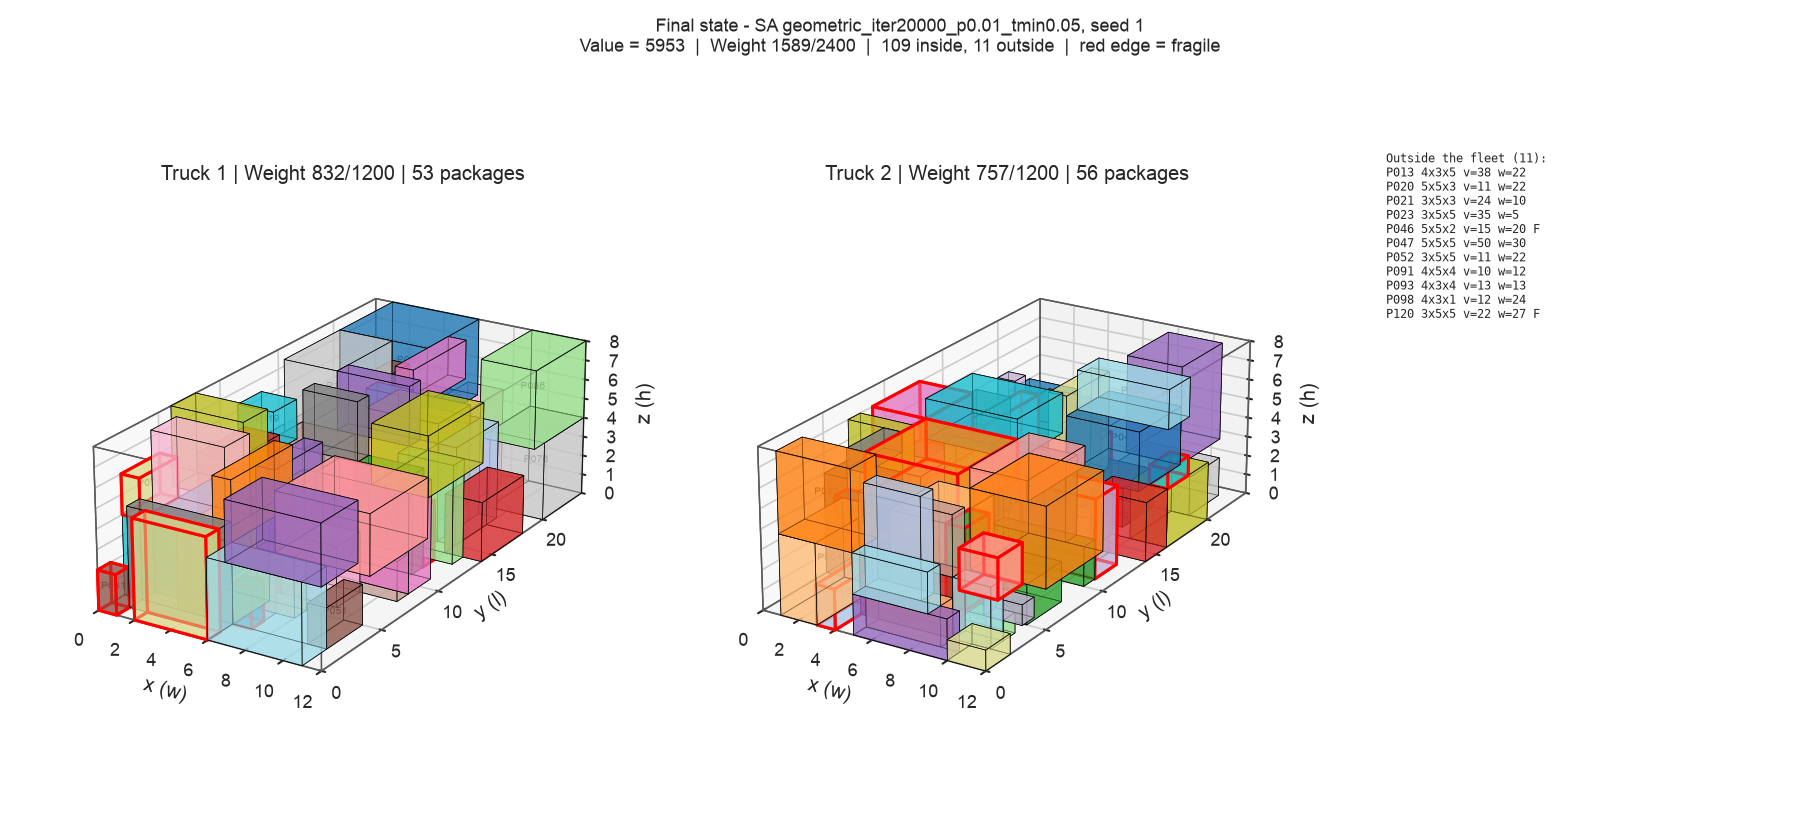
\includegraphics[width=\textwidth]{sa/large_trucks2/geometric_iter20000_p0.01_tmin0.05/seed1/final.png}
	\caption{\textit{State} akhir SA dengan dua truk (instans \textit{large}, \textit{seed} 1)}
	\label{fig:multitruck}
\end{figure}

Dengan dua truk, total \textit{value} yang diangkut naik 14--19\% untuk HC dan SA.
Kenaikannya tidak 100\% karena sebagian besar paket bernilai tinggi sudah terangkut
oleh satu truk. Pada \textit{large}, batasnya bukan lagi berat (1589 dari 2400 pada
Gambar~\ref{fig:multitruck}), melainkan volume dan geometri: paket yang tersisa di luar
umumnya berukuran besar dengan \textit{value} kecil. HC \textit{steepest} dan SA kini
hanya 2--4\% dari batas atas. Urutan kinerja algoritma tetap sama seperti pada satu
truk: SA dan HC \textit{steepest} unggul, HC \textit{stochastic} sedikit di bawahnya
(gap 7\%), sedangkan GA tertinggal jauh karena alasan yang sama
(Subbab~\ref{sec:ga-analisis}). Durasi SA
dan GA hanya naik sedikit, karena biaya per iterasi bergantung pada banyak paket di
setiap truk, bukan pada banyak truk.

\section{Analisis}

\begin{table}[H]
	\centering
	\caption{Perbandingan konfigurasi terbaik tiap algoritma (rata-rata 3 \textit{run})}
	\label{tab:compare}
	\begin{tabular}{l l r r r}
		\toprule
		\textbf{Instans} & \textbf{Algoritma} & \textbf{Akhir} & \textbf{Gap (\%)} & \textbf{Durasi (s)} \\
		\midrule
		\multirow{4}{*}{\textit{small}}  & HC \textit{steepest} & 680,7 & 7,3 & 0,29 \\
		& HC \textit{random-restart} & 712,7 & 2,9 & 1,21 \\
		& SA (20.000 iterasi) & \textbf{734,0} & \textbf{0,0} & 4,63 \\
		& GA (pop. 50, gen. 200) & 698,3 & 4,9 & 1,00 \\
		\midrule
		\multirow{5}{*}{\textit{medium}} & HC \textit{steepest} & 2213,7 & 7,1 & 53,51 \\
		& HC \textit{random-restart} & 2260,7 & 5,2 & 120,72 \\
		& SA (20.000 iterasi, $p_0=0{,}01$) & 2233,3 & 6,3 & 23,04 \\
		& SA (40.000 iterasi, $p_0=0{,}8$) & \textbf{2262,3} & \textbf{5,1} & 37,29 \\
		& GA (pop. 50, gen. 200) & 1477,7 & 38,0 & 0,67 \\
		\midrule
		\multirow{4}{*}{\textit{large}}  & HC \textit{steepest} & 5205,7 & 7,6 & 693,51 \\
		& HC \textit{random-restart} & \textbf{5261,7} & \textbf{6,6} & 1683,70 \\
		& SA (20.000 iterasi, \textit{ratio bias} 0,2) & 5076,3 & 9,9 & 21,30 \\
		& GA (pop. 100, gen. 100) & 2265,7 & 59,8 & 10,70 \\
		\bottomrule
	\end{tabular}
\end{table}

\subsection{Seberapa dekat dengan optimum global?}

Pada instans \textit{small}, SA mencapai 734 pada ketiga \textit{run}. Nilai ini sama
dengan batas atas, sehingga hasil SA \emph{terbukti} merupakan optimum global.
HC \textit{random-restart} tertinggal 2,9\% dan GA 4,9\%. Pada \textit{medium} dan
\textit{large}, HC dan SA berada 5--10\% di bawah batas atas (HC \textit{stochastic}
12--18\%). Angka ini merupakan
batas atas jarak, karena batas atas \textit{knapsack} mengabaikan geometri:
kombinasi paket yang muat berdasarkan berat dan volume belum tentu dapat disusun
tanpa celah, tanpa melayang, dan tanpa bertumpu pada paket \textit{fragile}.
Jarak sebenarnya ke optimum global kemungkinan lebih kecil.

GA tertinggal jauh pada \textit{medium} (38\%) dan \textit{large} (60\%). Penyebabnya
dibahas pada Subbab~\ref{sec:ga-analisis}.

\subsection{Perbandingan antaralgoritma}

\begin{itemize}
	\item \textbf{HC \textit{steepest-ascent}} cepat naik pada awal pencarian
	(Gambar~\ref{fig:hc-curve}), tetapi berhenti di \textit{local optimum} setelah
	7--65 iterasi. Hasilnya sudah cukup baik karena setiap langkah memilih yang terbaik
	dari ribuan tetangga.
	\item \textbf{HC \textit{stochastic}} hasilnya 0,5--11\% di bawah \textit{steepest}
	(gap 8--18\%) dengan waktu lebih singkat (0,1 detik di \textit{small}, 19 detik di
	\textit{medium}, dan 10 menit di \textit{large}). Langkahnya acak di antara tetangga
	yang lebih baik, bukan yang terbaik, sehingga setiap langkah naik lebih sedikit dan
	puncak yang dicapai umumnya lebih rendah. Pada \textit{large}, dua dari tiga
	\textit{run} berhenti karena \texttt{max\_iterations}=100, sehingga hasilnya masih
	dapat naik dengan iterasi lebih banyak.
	\item \textbf{HC \textit{sideways move}} tidak lebih baik daripada \textit{steepest}.
	Semua \textit{run} berhenti karena batas \textit{sideways move}. Artinya banyak
	\textit{plateau} (misalnya rotasi atau \textit{swap} paket di luar truk yang tidak
	mengubah nilai), tetapi berjalan di \textit{plateau} jarang menemukan jalan naik.
	\item \textbf{HC \textit{random-restart}} adalah varian HC terbaik dan paling konsisten,
	dengan biaya waktu beberapa kali lipat \textit{steepest} karena setiap
	\textit{restart} adalah satu pendakian penuh.
	\item \textbf{SA} terbaik di \textit{small}, setara HC \textit{random-restart} di
	\textit{medium} bila diberi 40.000 iterasi, dan sedikit di bawahnya di \textit{large}.
	Keunggulannya adalah waktu: puluhan detik dibanding puluhan menit HC pada \textit{large}.
	\item \textbf{GA} terburuk pada instans sedang dan besar meskipun waktunya singkat.
\end{itemize}

\subsection{Perbandingan durasi}

Biaya HC \textit{steepest} dan \textit{sideways} per iterasi sebanding dengan banyak
tetangga, yaitu $O(n^2)$ \textit{swap} ditambah $O(n^2)$ \textit{move} ke \textit{extreme
point}. Setiap tetangga juga di-\textit{repair}, yang biayanya kuadratik terhadap banyak
paket di truk. Karena itu waktunya tumbuh sangat cepat: sekitar 0,3 detik di
\textit{small}, 50 detik di \textit{medium}, dan 10--16 menit di \textit{large}.
\textit{Random-restart} sekitar 2--2,5 kali \textit{steepest}. HC \textit{stochastic}
hanya memeriksa seluruh tetangga ketika 50 tetangga acak tidak memberi perbaikan.
Pada satu \textit{run} \textit{medium}, hal ini terjadi pada 16 dari 36 iterasi dan
menghabiskan 98\% waktunya. Karena itu durasinya lebih singkat daripada
\textit{steepest}, tetapi tumbuh dengan cara yang sama terhadap ukuran instans.
Sebaliknya, SA dan GA hanya
menilai satu tetangga per iterasi atau per anak, sehingga biayanya hampir linear
terhadap banyak iterasi (Tabel~\ref{tab:sa-params}: 2.500 iterasi 1,7 detik, 40.000
iterasi 37 detik). GA paling cepat karena total anak yang dievaluasi hanya
populasi $\times$ generasi (paling banyak 10.000).

% TODO: hapus catatan ini jika eksperimen SA dijalankan ulang pada mesin yang sama dengan HC dan GA.
Catatan: eksperimen SA dijalankan pada waktu yang berbeda dari eksperimen HC dan GA.
Pengukuran ulang satu \textit{run} SA \textit{medium} 20.000 iterasi pada mesin yang
sama dengan HC hanya memerlukan sekitar 3 detik (Tabel~\ref{tab:sa-runs} mencatat
sekitar 23 detik). Karena itu, perbandingan durasi antaralgoritma dibaca sebagai
orde besaran. Kesimpulan bahwa HC jauh lebih lambat daripada SA pada instans besar
tidak berubah.

\subsection{Konsistensi hasil}

SA pada \textit{small} memberikan hasil identik di ketiga \textit{run}. Pada
\textit{medium} dan \textit{large}, HC \textit{random-restart} paling konsisten
(simpangan baku 7 dan 46), disusul SA (21 dan 42--75) dan HC \textit{steepest}.
HC \textit{stochastic} kurang konsisten (simpangan baku 54--123) karena langkahnya
dipilih secara acak, dan GA paling tidak konsisten. Simpangan baku GA mencapai
245 pada \textit{large}, karena hasilnya sangat bergantung pada individu awal terbaik
yang kebetulan terbentuk.

\subsection{Pengaruh parameter Simulated Annealing}

\begin{itemize}
	\item \textbf{Banyak iterasi} adalah parameter paling berpengaruh: nilai akhir naik
	dari 1985,7 (2.500 iterasi) menjadi 2262,3 (40.000 iterasi). Frekuensi \textit{stuck}
	ikut naik, karena dengan jadwal yang lebih panjang lebih banyak waktu dihabiskan
	pada suhu rendah.
	\item \textbf{$p_0$ kecil (0,01)} memberi hasil terbaik pada 10.000 iterasi. Dengan
	$p_0$ besar, sebagian besar iterasi awal terbuang untuk menerima langkah buruk.
	Karena setiap \textit{state} sudah di-\textit{repair} menjadi valid, sehingga eksplorasi
	berlebihan tidak diperlukan.
	\item \textbf{Jadwal geometrik} jauh lebih baik daripada linear (2187,7 vs 1755,7).
	Jadwal linear mempertahankan suhu tinggi terlalu lama dan baru dingin di akhir,
	sehingga waktu untuk memperbaiki solusi sangat sedikit.
	\item \textbf{$T_{\min}$ kecil} lebih baik. Dengan $T_{\min}=5$, langkah memburuk masih
	sering diterima di akhir, sehingga solusi tidak sempat ``mengeras''.
	\item \textbf{\textit{Ratio bias}} sedikit menaikkan rata-rata, yaitu +0,6\% di
	\textit{medium} dan +2,0\% di \textit{large} untuk bias 0,2.
\end{itemize}

\subsection{Pengaruh populasi dan generasi pada Genetic Algorithm}
\label{sec:ga-analisis}

Pada \textit{small} dan \textit{medium}, menambah generasi (50 $\rightarrow$ 200) dan
menambah populasi (20 $\rightarrow$ 100) sama-sama menaikkan nilai akhir. Pada
\textit{medium} nilainya naik dari 1221,7 ke 1477,7 untuk generasi dan dari 1220,0 ke
1422,7 untuk populasi. Kurva pada Gambar~\ref{fig:ga-compare} masih naik di akhir,
sehingga GA belum konvergen. Durasi naik linear terhadap populasi $\times$ generasi.
Pada \textit{large}, pengaruh keduanya hampir tertutup oleh variansi: banyak
\textit{run} tidak pernah melampaui individu terbaik generasi ke-0 (kolom ``Gen.
terbaik'' bernilai 0 pada Tabel~\ref{tab:ga-runs}).

Rendahnya kinerja GA disebabkan oleh operator \textit{crossover}. \textit{Single-point
crossover} menggabungkan koordinat paket dari dua susunan yang tidak berhubungan.
Posisi yang baik pada satu induk hanya bermakna relatif terhadap paket lain di susunan
induk itu, sehingga anak umumnya berisi banyak paket yang bertumpuk. \textit{Repair}
kemudian mengeluarkan paket-paket tersebut. Pengukuran tambahan pada 200 pasangan induk
acak dari populasi awal menunjukkan bahwa anak (setelah \textit{repair}) lebih baik
daripada induk terbaiknya hanya pada 8\% (\textit{small}), 6\% (\textit{medium}), dan
2\% (\textit{large}) kasus. Perbaikan nilai praktis hanya berasal dari mutasi, yaitu
satu langkah per anak dengan peluang 0,2. Jumlah ini jauh lebih sedikit daripada
puluhan ribu langkah SA. Selain itu, populasi awal acak setelah \textit{repair} hanya
berisi sekitar separuh paket yang semula dimasukkan, sehingga titik awal GA rendah.
Representasi yang cocok untuk \textit{crossover} versi salindia (\textit{string} dengan
gen yang independen, seperti 8-\textit{queens}) tidak cocok untuk persoalan
\textit{packing} yang gennya saling bergantung secara geometris.
